% Add these packages in the preamble:
% \usepackage{xcolor}
% \usepackage[normalem]{ulem}

\section{Methodology}
\label{sec:methodology}

This section describes the methodology used to evaluate SSHv2, SSH3, and Mosh under Agent-Like interactive terminal workloads.

\subsection{Workload Design}
\label{subsec:application-workloads}

\begin{figure}[t]
\centering
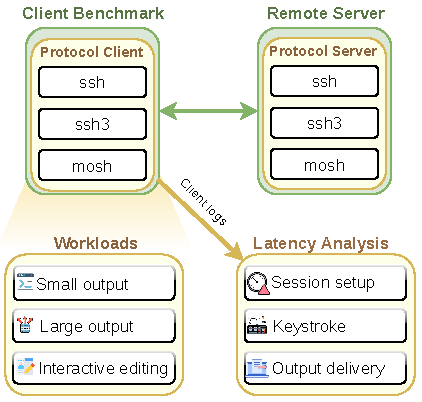
\includegraphics[width=0.9\columnwidth]{figs/workload.pdf}
\caption{Benchmark workload design and protocol performance metrics.}
\label{fig:workload}
\end{figure}

Figure~\ref{fig:workload} illustrates the benchmark workflow used in this study. In each run, the benchmark client selects the client implementation for the evaluated protocol. It uses \texttt{OpenSSH-Client} for SSHv2, \texttt{ssh3} for SSH3, and \texttt{mosh} for Mosh, with the Mosh session bootstrapped via \texttt{ssh}. The selected client then connects to the corresponding server implementation on the remote server: \texttt{sshd}, \texttt{ssh3-server}, or \texttt{mosh-server}. We select commonly used commands in remote shell environments, including system administration tasks, CI/CD workflows, container logs inspection, and interactive editing. These commands are divided into three workloads based on output size and interaction characteristics, allowing each workload to isolate a specific aspect of protocol performance.

\paragraph{Small output commands}
Workload 1 (W1) consists of four commands that produce outputs under 1 KB: \texttt{ls}, \texttt{df -h}, \texttt{grep -n root /etc/passwd}, and \texttt{git status}. Because these commands produce small outputs.

\paragraph{Large output commands}
Workload 2 (W2) consists of four commands that generate outputs in the 2-10 MB range: \texttt{yes | head -c N}, \texttt{seq}, \texttt{cat}, and \texttt{docker logs}. These commands emulate large terminal output streams such as system logs, container logs, build results, or test results. 

\paragraph{Interactive editing}
Workload 3 (W3) consists of \texttt{shell}, \texttt{vim}, and \texttt{nano}, and evaluates character-level responsiveness when the user types continuously. This workload includes two variants: a single-pane variant (1P) and a five-pane variant (5P). In the 5P variant, pane 0 receives the keystroke probe sequence, while panes 1-4 generate background redraw load. This workload allows us to observe how protocol performance diverges under concurrent terminal activity.

\subsection{Measurement Metrics and Analysis}
\label{subsec:measurement-analysis}

Figure~\ref{fig:workload} provides the deployment context for the client-side measurements described. The metrics below are computed from terminal events observed at the benchmark client.

Since all latency metrics follow the same event difference structure, we define a general latency metric as
\begin{equation}
L_m = t_{\mathrm{obs}}^{m} - t_{\mathrm{init}}^{m},
\end{equation}
where $m$ identifies the measurement type, $t_{\mathrm{init}}^{m}$ is the client-side timestamp when the measured action is initiated, and $t_{\mathrm{obs}}^{m}$ is the client-side timestamp when the corresponding terminal event becomes visible.

After the session is ready, the client runs the workloads. The benchmark records protocol logs and workload observations to analyze three metrics: session setup latency, output delivery latency, and keystroke responsiveness. Session setup latency captures how long it takes to establish an interactive shell session. Output delivery latency captures how long it takes for command output to become visible at the client. Keystroke responsiveness captures how long it takes for a typed character to appear on the client terminal. We instantiate $L_m$ for these latency analysis categories, as shown in Figure~\ref{fig:workload}. Session setup latency ($L_{\mathrm{setup}}$) is measured from the moment the benchmark client starts establishing a remote shell session until the first shell prompt appears. Output delivery latency ($L_{\mathrm{out}}$) is measured for both W1 and W2, from command transmission to completion marker visibility after the command output is produced, W1 uses small output commands, whereas W2 uses large output commands. Keystroke responsiveness is measured for W3 as input to visible latency in the 1P ($L_{\mathrm{input}}$) and 5P ($L_{\mathrm{input}}^{\mathrm{5pane}}$) settings, from probe send to character visibility at the client. In the 5P case, pane 0 is observed while panes 1-4 generate background redraw load. For Mosh, $L_{\mathrm{out}}$ reflects observable terminal completion rather than byte complete delivery, and $L_{\mathrm{input}}$ reflects predictive local echo.

To measure output completeness, we remove ANSI escape sequences \cite{ECMA48}, including color formatting and cursor control sequences. This keeps the comparison focused on textual content rather than terminal rendering artifacts. The cleaned client output is then compared with a reference output obtained from three SSH runs without a pseudo-terminal (no-PTY). For each sample, the output completeness percentage is computed from the observed output size and the reference size, capped at 100\%. We report the average and minimum output completeness percentage for each protocol, scenario, workload, and command combination over all non-warmup samples.

For each sample, we record the measurement results, including execution status, session setup latency, latency and output completeness percentage for W1 and W2, and keystroke latency for W3. In the aggregate analysis, we report the mean, standard deviation, and 95\% confidence interval for each latency metric.